\documentclass[usenames,dvipsnames,tikz]{standalone}
%\usepackage{xcolor}
%\definecolor{tLightGreen1}{HTML}{B7F385} %tikz color
%\definecolor{tLightOrange1}{HTML}{FFCD4F} %tikz color
%\colorlet{tLightGreen}{LimeGreen!70!OliveGreen!45!White}
%\colorlet{tLightOrange}{Dandelion!65!White}
\definecolor{tLightPink}{HTML}{FFD4EB} %tikz color
\definecolor{tLightBlue}{HTML}{CEF0FF} %tikz color
\colorlet{tRed}{Red}
%\usepackage{tikz}
%\usepackage{standalone}
\begin{document}
	
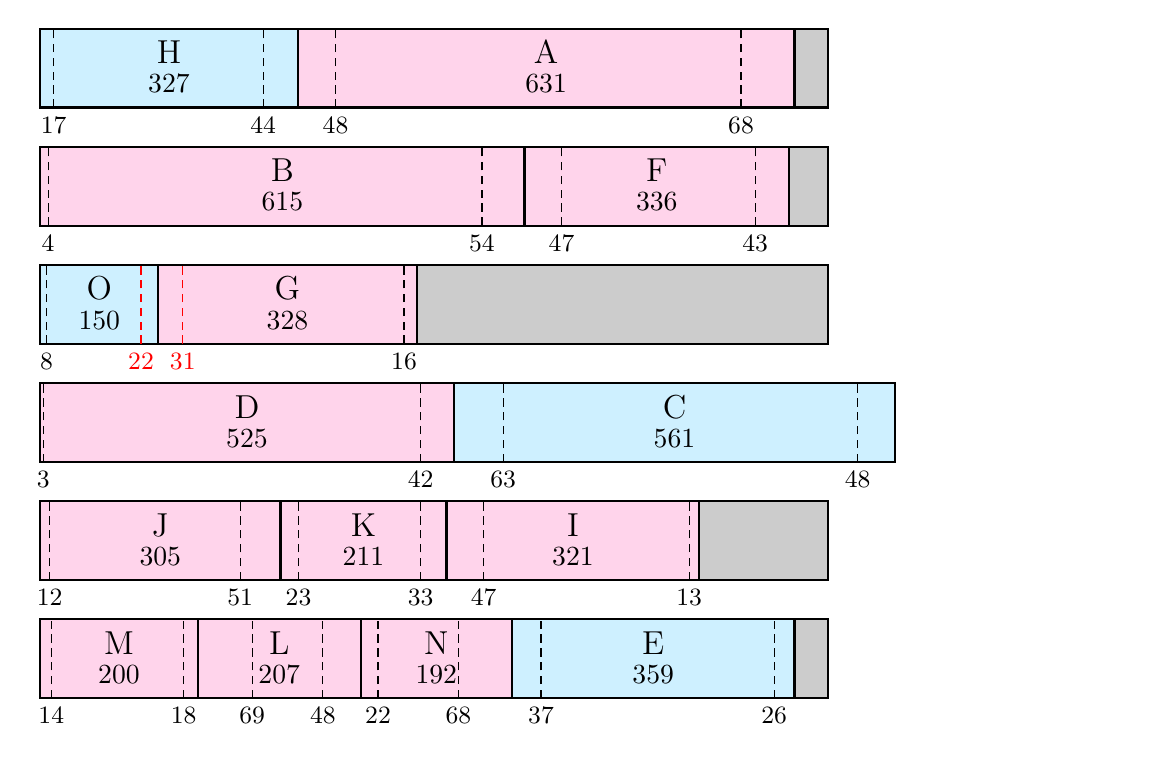
\begin{tikzpicture}
%\draw [help lines] (-1,-2) grid (13,11);

%blank rectangle to match offspring2:
\draw [thick, white] (0, 4.5) rectangle (13.99, 5.5);

% H,A, 327, 631 (17-44, 48-68) H FROM OTHER PARENT
\path [fill=tLightBlue] (0,7.5) rectangle (3.27,8.5);
\path [fill=tLightPink] (3.27,7.5) rectangle (9.58,8.5);
\draw [thick] (0,7.5) rectangle (10, 8.5);
\draw [thick] (3.27,7.5) -- (3.27, 8.5); % H FROM OTHER PARENT
\draw [thick] (9.58,7.5) -- (9.58, 8.5);
\filldraw[fill=black!20!white, draw=black, thick] (9.58,7.5) rectangle (10,8.5);
\draw [densely dashed] (0.17,7.5) -- (0.17,8.5);
\draw [densely dashed] (2.83,7.5) -- (2.83,8.5);
\draw [densely dashed] (3.75,7.5) -- (3.75,8.5);
\draw [densely dashed] (8.9,7.5) -- (8.9,8.5);
\node at (1.635,7.8) {$327$};
\node at (6.425,7.8) {$631$};
\node at (1.635,8.2) {\large H};
\node at (6.425,8.2) {\large A};
\node [below] at (0.17,7.5) {\small$17$};
\node [below] at (2.83,7.5) {\small$44$};
\node [below] at (3.75,7.5) {\small$48$};
\node [below] at (8.9,7.5) {\small$68$};

% B, F, 615, 336 (4-54, 47-43)
\path [fill=tLightPink] (0,6) rectangle (9.51,7);
\draw [thick] (0,6) rectangle (10, 7);
\draw [thick] (6.15,6) -- (6.15,7);
\draw [thick] (9.51,6) -- (9.51,7);
\filldraw[fill=black!20!white, draw=black, thick] (9.51,6) rectangle (10,7);
\draw [densely dashed] (0.1,6) -- (0.1,7);
\draw [densely dashed] (5.61,6) -- (5.61,7);
\draw [densely dashed] (6.62,6) -- (6.62,7);
\draw [densely dashed] (9.08,6) -- (9.08,7);
\node at (3.075,6.3) {$615$};
\node at (7.83,6.3) {$336$};
\node at (3.075,6.7) {\large B};
\node at (7.83,6.7) {\large F};
\node [below] at (0.1,6) {\small$4$};
\node [below] at (5.61,6) {\small$54$};
\node [below] at (6.62,6) {\small$47$};
\node [below] at (9.08,6) {\small$43$};


% O, G, 150, 328 (8-22 X 31-16) (VSC NOT MET) O FROM OTHER PARENT
\path [fill=tLightBlue] (0,4.5) rectangle (1.5,5.5);
\path [fill=tLightPink] (1.5,4.5) rectangle (4.78,5.5);
\draw [thick] (0,4.5) rectangle (10, 5.5);
\draw [thick] (1.5,4.5) -- (1.5,5.5); % O FROM OTHER PARENT
\draw [thick] (4.78,4.5) -- (4.78,5.5);
\filldraw[fill=black!20!white, draw=black, thick] (4.78,4.5) rectangle (10,5.5);
\draw [densely dashed] (0.08,4.5) -- (0.08,5.5);
\draw [densely dashed, tRed] (1.28,4.5) -- (1.28,5.5);
\draw [densely dashed, tRed] (1.81,4.5) -- (1.81,5.5);
\draw [densely dashed] (4.62,4.5) -- (4.62,5.5);
\node at (0.75,4.8) {$150$};
\node at (3.14,4.8) {$328$};
\node at (0.75,5.2) {\large O};
\node at (3.14,5.2) {\large G};
\node [below] at (0.08,4.5) {\small$8$};
\node [below] at (1.28,4.5) {\textcolor{tRed}{\small$22$}};
\node [below] at (1.81,4.5) {\textcolor{tRed}{\small$31$}};
\node [below] at (4.62,4.5) {\small$16$};


% D, C 525, 561 (3-42, 63-48) (OVERFULL) C FROM OTHER PARENT
\path [fill=tLightPink] (0,3) rectangle (5.25,4);
\path [fill=tLightBlue] (5.25,3) rectangle (10.86,4);
\draw [thick] (0,3) rectangle (10.86, 4);
\draw [thick] (5.25,3) -- (5.25,4);
\draw [thick] (10.86,3) -- (10.86,4); % C FROM OTHER PARENT
%\filldraw[fill=black!20!white, draw=black, thick] (8.52,3) rectangle (10,4);
\draw [densely dashed] (0.04,3) -- (0.04,4);
\draw [densely dashed] (4.83,3) -- (4.83,4);
\draw [densely dashed] (5.88,3) -- (5.88,4);
\draw [densely dashed] (10.38,3) -- (10.38,4);
\node at (2.625,3.3) {$525$};
\node at (8.055,3.3) {$561$};
\node at (2.625,3.7) {\large D};
\node at (8.055,3.7) {\large C};
\node [below] at (0.04,3) {\small$3$};
\node [below] at (4.83,3) {\small$42$};
\node [below] at (5.88,3) {\small$63$};
\node [below] at (10.38,3) {\small$48$};


% J, K, I, 305, 211, 321 (12-51, 23-33, 47-13)
\path [fill=tLightPink] (0,1.5) rectangle (8.37,2.5);
\draw [thick] (0,1.5) rectangle (10, 2.5);
\draw [thick] (3.05,1.5) -- (3.05,2.5);
\draw [thick] (5.16,1.5) -- (5.16,2.5);
\draw [thick] (8.37,1.5) -- (8.37,2.5);
\filldraw[fill=black!20!white, draw=black, thick] (8.37,1.5) rectangle (10,2.5);
\draw [densely dashed] (0.12,1.5) -- (0.12,2.5);
\draw [densely dashed] (2.54,1.5) -- (2.54,2.5);
\draw [densely dashed] (3.28,1.5) -- (3.28,2.5);
\draw [densely dashed] (4.83,1.5) -- (4.83,2.5);
\draw [densely dashed] (5.63,1.5) -- (5.63,2.5);
\draw [densely dashed] (8.24,1.5) -- (8.24,2.5);
\node at (1.525,1.8) {$305$};
\node at (4.105,1.8) {$211$};
\node at (6.765,1.8) {$321$};
\node at (1.525,2.2) {\large J};
\node at (4.105,2.2) {\large K};
\node at (6.765,2.2) {\large I};
\node [below] at (0.12,1.5) {\small$12$};
\node [below] at (2.54,1.5) {\small$51$};
\node [below] at (3.28,1.5) {\small$23$};
\node [below] at (4.83,1.5) {\small$33$};
\node [below] at (5.63,1.5) {\small$47$};
\node [below] at (8.24,1.5) {\small$13$};


% M, L, N, E, 200, 207, 192, 359 (14-18, 69-48, 22-68, 37-26) E FROM OTHER PARENT
\path [fill=tLightPink] (0,0) rectangle (5.99,1);
\path [fill=tLightBlue] (5.99,0) rectangle (9.58,1);
\draw [thick] (0,0) rectangle (10, 1);
\draw [thick] (2,0) -- (2,1);
\draw [thick] (4.07,0) -- (4.07,1);
\draw [thick] (5.99,0) -- (5.99,1);
\draw [thick] (9.58,0) -- (9.58,1); % E FROM OTHER PARENT
\filldraw[fill=black!20!white, draw=black, thick] (9.58,0) rectangle (10,1);
\draw [densely dashed] (0.14,0) -- (0.14,1);
\draw [densely dashed] (1.82,0) -- (1.82,1);
\draw [densely dashed] (2.69,0) -- (2.69,1);
\draw [densely dashed] (3.59,0) -- (3.59,1);
\draw [densely dashed] (4.29,0) -- (4.29,1);
\draw [densely dashed] (5.31,0) -- (5.31,1);
\draw [densely dashed] (6.36,0) -- (6.36,1);
\draw [densely dashed] (9.32,0) -- (9.32,1);
\node at (1,0.3) {$200$};
\node at (3.035,0.3) {$207$};
\node at (5.03,0.3) {$192$};
\node at (7.785,0.3) {$359$};
\node at (1,0.7) {\large M};
\node at (3.035,0.7) {\large L};
\node at (5.03,0.7) {\large N};
\node at (7.785,0.7) {\large E};
\node [below] at (0.14,0) {\small$14$};
\node [below] at (1.82,0) {\small$18$};
\node [below] at (2.69,0) {\small$69$};
\node [below] at (3.59,0) {\small$48$};
\node [below] at (4.29,0) {\small$22$};
\node [below] at (5.31,0) {\small$68$};
\node [below] at (6.36,0) {\small$37$};
\node [below] at (9.32,0) {\small$26$};

%\node at (5, -1.5) {\huge{$\mathcal{S}_1$}};



\end{tikzpicture}
	
\end{document}